\chapter{Task Distribution in a Flat Organization\label{sec:work-distribution}}

\Gls{bureaucracy} is not the only explanation for patterns observed when people interact. How tasks get distributed in an organization is a confounding aspect.  This chapter describes a model of processes and tasks that involve coordination. 
The model is useful for distinguishing the effects of bureaucracy (distributed knowledge and distributed decision making) from the distribution of tasks in an organization.

The model of task distribution in an organization is sufficiently detailed to illustrate commonly observed situations, but is agnostic to the specific tasks or work roles. Improvements to the model intended to increase the realism could be made, but risk decreasing the clarity of the model.

\section{Assumptions in the Model of Task Distribution}

The model relies on a few concepts. These definitions are local to the numerical model and do not apply to the rest of the book.
\begin{itemize}
    \item Specialization: categories of ability. A person has a specialization; completing a task requires a specialization.
    \item Skill-level: a ranking of how quickly work can be done for a task. If a task requires a skill-level higher than a person has, then that person is unable to complete the task.
    \item Person: is a member of the organization, has specializations, has a skill-level per specialization, can receive tasks, and can engage with strangers in the organization. A person can complete one task at a time. A person can coordinate one task at a time. 
    \begin{itemize}
        \item Person's contact list: A person has a list of people they've previously given tasks to. When figuring out who to give a task to, they can review the list of people they already know. 
        \item Person's backlog: Each person maintains a queue of tasks to be done.
        \item Person's status: A person is either idle (not assigned a task), working on a task, or coordinating with other people. 
    \end{itemize}
    \item Organization: a set of people who can be assigned work. 
    \item Task: requires one specialization, has an associated minimum skill-level, and has an amount of time that the task takes. A task can only be worked on by one person at a time. 
    \item Process: comprised of one or more tasks.\footnote{See Wikipedia entry on 
    \index{Wikipedia!\href{https://en.wikipedia.org/wiki/Queueing_theory}{Queueing Theory}}
    \href{https://en.wikipedia.org/wiki/Queueing_theory}{Queueing Theory}.} Tasks in a process are worked on sequentially by people. A process is owned by one person who is either coordinating or working on the task.  Processes are independent.
\end{itemize}

In the model I'm using the word task instead of work because work is a Physics concept that applies when there is a product that is tangible and countable. Making tacos takes work; approving requests is a distinct concept because there is nothing tangible. For knowledge workers, which most bureaucrats are, the unit of tasking is attention-time spent on an issue.
Each participant in the organization has the same amount of attention-time to spend, but different specializations and skill-levels.

%The model is abstract so that is applicable to many contexts. 
%A simple process is a sequence of few tasks, and each task does not require significant specialization or skill-level.
%A complex process is a sequence of many tasks, and each task requires specialized skills, and the number of distinct specializations is high.

When a person is assigned a task they don't have the specialization for, or lack sufficient skill-level, then they have to find someone else in the organization who is capable of doing the task. 
In the numerical model the random selection of someone else who has the necessary specialization and skill-level is insensitive to the size of their backlog. This is reflects my experience in a large organization where the backlog visibility is not shared by anyone, so you merely add something to their backlog and hope they will get to it eventually.



The model relies on a process being a sequence of tasks. That might not be realistic when branching is part of a process (conditional branching or splitting).
Real processes feature branching in two senses. The first sense of branching is the conditional logic of if this else that
The second sense of branching is that a task be the initiation point of another process
However, in either of those two senses of branching, in practice the processes can be treated as isolated sequences of tasks.



The need for coordination blamed on the random delegation of task not being aligned but the skills and skill levels of the workers. 
But that only applies if the tasks are atomic and independent.

If the task are part of a process, and a person owns the process, and task in a process cannot be handled by one person, then coordination re-emerges as a requirement.


The distribution of skills and specializations of people in an organization is set by the hiring process.


Simplifying assumptions about what isn't in the numerical model:
\begin{itemize}
    \item There is nothing in the model about policies, decision making\footnote{For example, see ``To how many politicians should government be left?'' (2008). \href{https://arxiv.org/pdf/0804.2202.pdf}{https://arxiv.org/pdf/0804.2202.pdf}}, shared resources, or subjects of bureaucracy. 
    \item There's no hierarchy in the model. I am modeling people cooperating in an organization. Unlike the rest of the book, this model does not use the distinction of organizations being comprised of teams.
    \item People in the model don't get to initiate any task of their own volition. They work on tasks from their personal backlog, or from an infinite pool of tasks.
    \item People in the model don't get to refuse any task that is assigned to them for which they have the specialization and relevant skill-level.
    \item No overtime; every person gets the same amount of time to do work.
    \item No support staff; all infrastructure for communication and tasks works without failure.
    \item No dark patterns. Everyone does work assigned promptly and correctly.
    \item No turnover of staff during the simulation.
    \item No improvement of skill per person, or additional specialization.
\end{itemize}
The complexities above are not included in the model because the point of the model is to show what arises from simple constraints. 

Within the constraints there are improvements that could be made to the model.%, but are not expected to alter the conclusions:
The conclusions drawn from the model map to real-world organizations even without these features: 
\begin{itemize}
    \item Use realistic distributions (e.g., power law) instead of uniform distributions.
    \item When a person is not qualified to do a task, instead of searching randomly, search second-order contacts.
\end{itemize}

\section{Tasks and People}

Suppose the model is configured to simulate three specializations (A, B, C) and three skill-levels (1, 2, 3). 

\subsubsection{People}

A person with skill-level 3 in specialization A and skill-level 1 in specialization C would be labeled ``A3,C1'':

\begin{center}
\begin{tabular}{c|c|c|c|}
&\multicolumn{3}{c}{\footnotesize Specializations}\\
\hline
& A & B & C \\
\hline
1 & X & & X \\
\hline
2 & X & & \\
\hline
3 & X & & \\
\hline
\end{tabular}
\end{center}

Because a person has skill-level three in specialization A, that means they can also work on tasks that require skill-level two or skill-level one.

People can be characterized by the depth and breadth of their skills. For example, a ``expert specialist'' (e.g.,~``B3") is good at one thing, while a ``general specialist" (e.g.,~``A1,B3,C1") has \href{https://en.wikipedia.org/wiki/T-shaped_skills}{T-shaped skills}:

\begin{center}
Expert:
$\left\{
\begin{tabular}{c|c|c|c|}
&\multicolumn{3}{c}{\footnotesize Specializations}\\
%\hline
& A & B & C \\
\cline{2-4}
1 & &  X &  \\
\cline{2-4}
2 & & X & \\
\cline{2-4}
3 & & X & \\
\cline{2-4}
\end{tabular}
\right.$
\qquad
Generalist Expert:
$\left\{
\begin{tabular}{c|c|c|c|}
& \multicolumn{3}{c}{\footnotesize Specializations}\\
%\hline
& A & B & C \\
\cline{2-4}
1 & X &  X & X \\
\cline{2-4}
2 & & X & \\
\cline{2-4}
3 & & X & \\
\cline{2-4}
\end{tabular}
\right.$
\end{center}

A generalist (here~``A1,B1,C1") is not an expert at anything, but capable in multiple specializations. A Unicorn (here a~``A3,B3,C3") can do everything well.
\begin{center}
Generalist:
$\left\{
\begin{tabular}{c|c|c|c|}
 & \multicolumn{3}{c}{\footnotesize Specializations}\\
%\hline
& A & B & C \\
\cline{2-4}
1 & X &  X & X \\
\cline{2-4}
 2 & &  & \\
\cline{2-4}
3 &  &  & \\
\cline{2-4}
\end{tabular}
\right.$
\qquad
Unicorn:
$\left\{
\begin{tabular}{c|c|c|c|}
& \multicolumn{3}{c}{\footnotesize Specializations}\\
%\hline
   & A & B & C \\
\cline{2-4}
 1 & X & X & X \\
\cline{2-4}
 2 & X & X & X \\
\cline{2-4}
 3 & X & X & X \\
\cline{2-4}
\end{tabular}
\right.$
\end{center}


There are many more unskilled specialists (e.g.,~``A1'') than Unicorns
\begin{center}
Unskilled Specialist:
$\left\{
\begin{tabular}{c|c|c|c|}
& \multicolumn{3}{c}{\footnotesize Specializations}\\
%\hline
   & A & B & C \\
\cline{2-4}
 1 & X &   &  \\
\cline{2-4}
 2 &   &   & \\
\cline{2-4}
 3 &   &   & \\
\cline{2-4}
\end{tabular}
\right.$
\end{center}

\subsection{Tasks and Processes}

A task that requires skill-level 2 in specialization B would be labeled ``B2.''
%\begin{center}
%\begin{tabular}{|c|c|c|}
%\multicolumn{3}{c}{\footnotesize Specializations}\\
%\hline
%A & B & C \\
%\hline
% &   &  \\
%\hline
% & X & \\
%\hline
% & & \\
%\hline
%\end{tabular}
%\end{center}
The assumption that a task requires one specialization is based on the idea that a process can be broken into atomic units. 

If a task requires specialization skill level 2 and takes 10 minutes, then
\begin{itemize}
    \item A person with skill-level 2 completes the task in 10 minutes.
    \item A person with skill-level 3 completes the task in  7 minutes (=10/(3/2)).
    \item A person with skill-level 1 is unable to complete the task.
\end{itemize}


A process is a sequence of tasks. For example, the list ``B2:10, A1:5, C3:7" describes three tasks: 
\begin{enumerate}
    \item Task requiring specialization B and skill-level 2; duration of 10 minutes.
    \item Task requiring specialization A and skill-level 1; duration of 5 minutes.
    \item Task requiring specialization C and skill-level 3; duration of 7 minutes.    
\end{enumerate}

\section{Configurations of the Model}

\subsection*{Scenario: Everyone is an A1}

Suppose every person in the organization is an A1 and every task is an A1.

\begin{center}
\begin{tabular}{c|c|}
%\cline{2}
  & A \\
\cline{2-2}
1 & X \\
\cline{2-2}
\end{tabular}
\end{center}

As a consequence of this configuration, no coordination is required.
\begin{itemize}
    \item The number of people each person knows is irrelevant.
    \item This configuration yields the maximum throughput tasks for the organization.
    \item Adding more people increases the throughput.
\end{itemize}
The benefits of every member being able to do every task is the model 
\index{Wikipedia!\href{https://en.wikipedia.org/wiki/Adhocracy}{adhocracy}}
\href{https://en.wikipedia.org/wiki/Adhocracy}{adhocracy} advocates.

%TODO: Plot throughput versus organization size 


\subsection*{Scenario: A1,B1 or A1,B0 or A0,B1 or A0,B0\\with (task duration = coordination duration)\\with no social circle}

The first non-trivial scenario is when not every member of an organization can do every task. There are two specializations (A, B) and one skill level: 

\begin{center}
\begin{tabular}{c|c|c|}
%\cline{2-3}
  & A & B \\
\cline{2-3}
1 & X &   \\
\cline{2-3}
\end{tabular}
\quad and \quad
\begin{tabular}{c|c|c|}
%\cline{2-3}
  & A & B \\
\cline{2-3}
1 &   & X \\
\cline{2-3}
\end{tabular}
\quad and \quad
\begin{tabular}{c|c|c|}
%\cline{2-3}
  & A & B \\
\cline{2-3}
1 & X & X \\
\cline{2-3}
\end{tabular}
\quad and \quad
\begin{tabular}{c|c|c|}
%\cline{2-3}
  & A & B \\
\cline{2-3}
1 &   &   \\
\cline{2-3}
\end{tabular}
\end{center}
In this configuration, the person qualified as A1,B1 is labeled a Unicorn -- they can do any task. Whether you consider inclusion of A0,B0 (a person who does does no work and can only coordinate) to be relevant depends on your personal experience. Most organizations label these members as ``managers.'' 

When a person does not have all the specializations, then a task randomly assigned to one person may need to be given to someone else in the organization. For example, if I am an A1 and am given a B1 task, I need to find a coworker who is either qualified as B1 or A1,B1. Sharing tasks among members of the organization requires coordination.

\begin{figure}
\centering
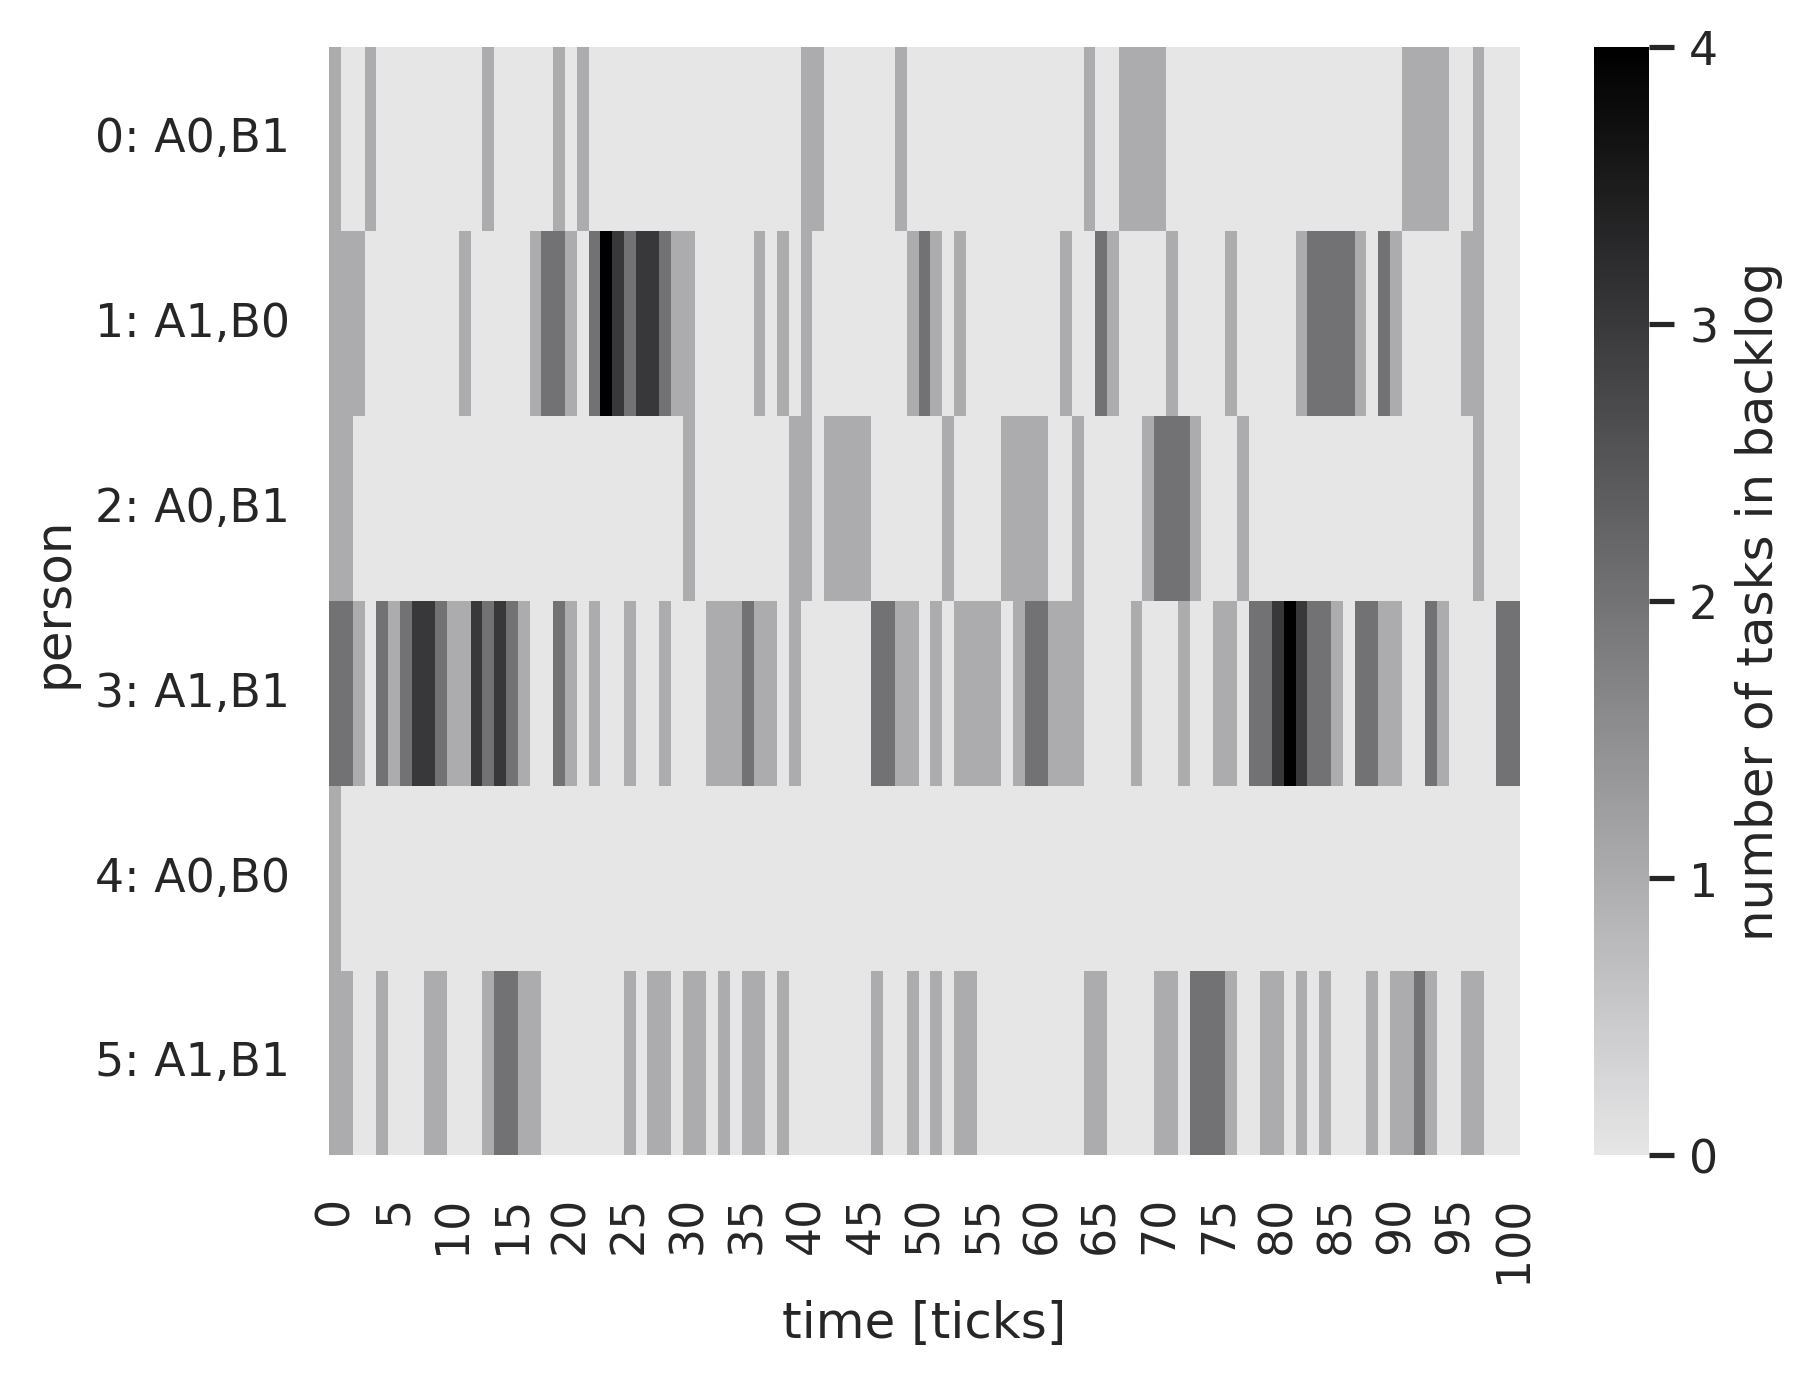
\includegraphics{images/task_distribution_backlog_length_per_person_simCount1_skills2_levels1_taskduration1_people6_social0_ticks100.png}
\caption{The length of each person's backlog (for 6 people) as a function of time. The backlog of person A0,B0}
\label{fig:task-distribution-backlog-length}
\end{figure}


Task throughput is a metric for comparing different configurations. Rather than count tasks per tick during steady-state, here we count number of tasks completed in 100 ticks. 

a metric of interest is the number of task per simulated tick as a function of the number of people present in the organization.


\begin{figure}
\centering
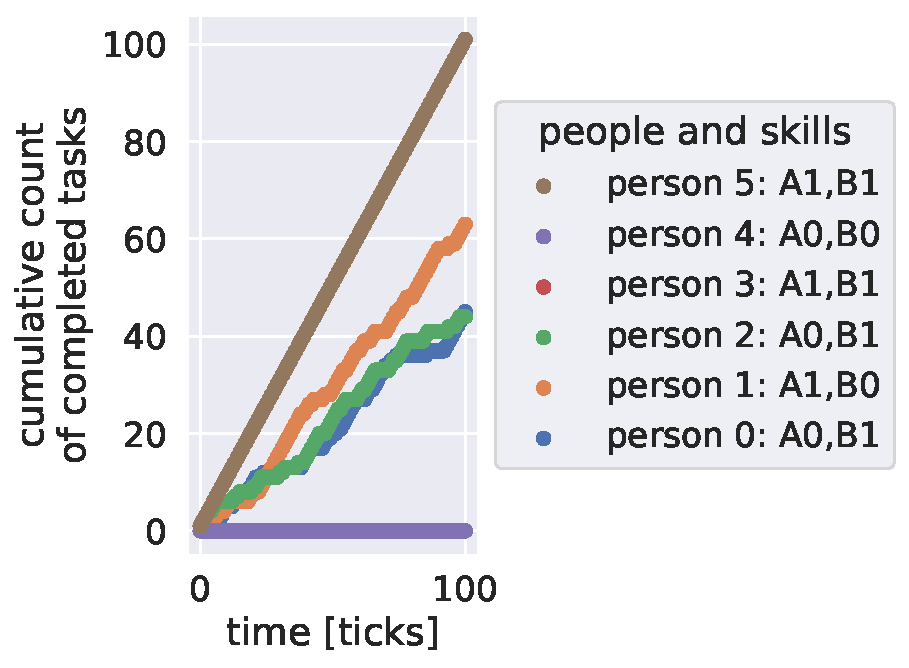
\includegraphics{images/task_distribution_tasks_per_person_simCount1_skills2_levels1_taskduration1_people6_social0_ticks100.pdf}
\caption{Tasks per person}
\label{fig:task-distribution-tasks-per-person}
\end{figure}

\begin{figure}
\centering
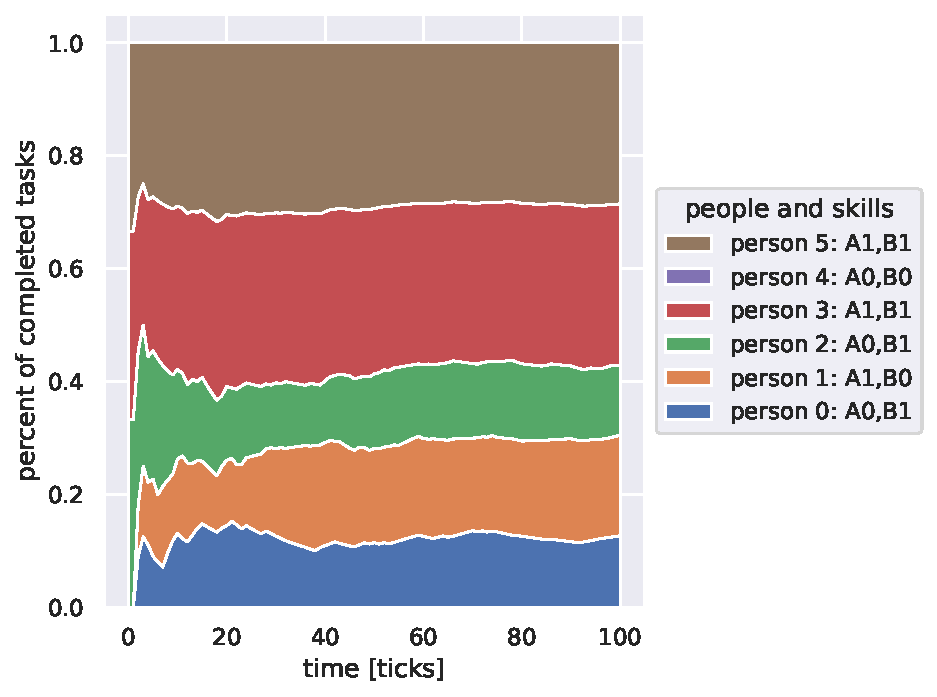
\includegraphics{images/task_distribution_percent_of_tasks_per_person_simCount1_skills2_levels1_taskduration1_people6_social0_ticks100.pdf}
\caption{Percentage}
\label{fig:task-distribution-percent-of-tasks}
\end{figure}

 
The reward for good work is more work.

coordination means lower throughput (with social size 0)

TODO: Plot throughput versus organization size 


\subsection*{Scenario: A1,B1 or A1,B0 or A0,B1 or A0,B0\\with (task duration = coordination duration)\\with social circle}

The amount of time a person assigned a task spends searching the organization depends on who else that person already knows. 

If I'm qualified as ``A1" and the task is ``B1," then I can give the task to a coworker who I know is qualified as ``B1." If I don't know anyone with the relevant specialization and skill-level, then I have to search the rest of the organization.
The amount of time spent searching depends on the number of people you know. 

With this feature in the model, we can look for a tipping point when the organization is larger than the size of each member's social circle. We expect a change in throughput when the organization exceeds Dunbar's number.

Result: social circle size matters to throughput 
Plot throughput versus social size for fixed organization size.

A person who is an A1,B1 will have no contact list because there is no handoff needed. A person who is A0,B0 will have a randomly populated contact list. A person who is A1,B0 will have a contact list populated with people who have B1.


% TODO: https://en.wikipedia.org/wiki/Little%27s_law


\subsection*{Scenario: A1,B1 or A1,B0 or A0,B1 or A0,B0\\with (task duration $>$ coordination duration)\\with no social circle}

Result: whether throughput is lower or higher than one person is sensitive to ratio of task:coord

Result: social circle size matters to throughput 

Result: reward for good work is more work 

\subsection*{}

A person who is an A3 B3 c3 will have no contact list because there is no handoff needed. A person who is a0 b0 c0 will have a randomly populated contact list. A person who is A3B0C0 will have a contact list populated with people who have non-zero skills in B and C

\section{to investigate}

The minimum throughput is no unicorns. What is the spread?

Does the system reach steady state? 
Or do task backlogs grow unbounded?

What is the relevance of unicorns who can do every task well for throughput or minimum task completion time?
(Characterization) What is the density of unicorns?



My guess is that under certain conditions, the simulated time is much greater than the task took time, which indicates that doing the work yourself would be quicker rather than distributing the work among an organization.
Why then would one distribute work among the organization?Because the specialization of skills is two diverse for anyone person to master everything. For example if you inspected your own meat for food safety, and monitor the emissions of a whole-fired power plan, and built your own semiconductor ships and built your own airplane, it might be quicker than distributing it among an organization of people with different skills.


The search time when the organization is smaller than a socialist goal is negligible, whereas when the organization is larger than their social circle the search time increases proportional to the number of people never organization. This is an obvious statement, but it indicates why larger organizations feel different than a small group of people working together who know each other
Hierarchy is not included in this numerical model, but it is one way of addressing this? Of how to coordinate outside of your social circle.



\section{So What?}

% source: https://graphthinking.blogspot.com/2023/02/prioritization-of-tasks.html

When there is more work than person hours, prioritization becomes critical. Without prioritization, tasks get started and do not get completed.

Prioritization requires sacrifice (what are you not doing) and induces risk (there is consequence to not doing things) and spends your reputation (not doing things effects other people).

There are two conditions under which prioritization becomes important. 
\begin{itemize}
    \item The amount of work is less than or equal to the amount of staff available and skill over the staff. Then prioritization is merely ordering of work.
    \item When work exceeds staff and skill-level per person, you won't get to everything as an oversubscribed person. Saying no is important but harms your reputation.
\end{itemize}


Prioritization strategies
\begin{itemize}
    \item Don't prioritize. Work on task as they are identified and don't complete anything because it gets interrupted by the next task
Static prioritization that is exclusive. Only work on one thing to the exclusion of everything else.
    \item Shifting prioritization (prioritization changes over time)
    \begin{itemize}
        \item Prioritization that evolves slower than task can be completed
        \item Prioritization that shifts faster than task can be completed is ineffective because it is indistinguishable from responding to task as they arise.
    \end{itemize}
    \item Proportional allocation for task prioritization. 10\% of your time for area one, 20\% of your time for two. 
\end{itemize}
